\section{Paper 9}
\subsection{\emph{"Similar Face Recognition Using the IE-CNN Model"}}

\begin{frame}{INTRODUCTION}
    Currently there are few datasets that provide a set of images with faces of 
    similar people, moreover there are few methods tested to be able to verify 
    the level of similarity. Two types of work are carried out in the following paper. 
    The first is based on proposing a procedure for creating a large dataset of 
    similar faces that requires a small amount of person-power to label the content. 
    In the second work, instead, an IE-CNN model is built which has the task 
    of improving the internal and external features of the face, increasing the 
    precision of face matching.
\end{frame}

\begin{frame}{RELATED WORK}
    Internal and external features are particularly important in recognizing a 
    subject. The proposed method uses both of them unlike the other 
    recognition algorithms. If used separately, the algorithm could associate 
    two different individuals with the same identity.
    \begin{figure}[h!]
        \centering
        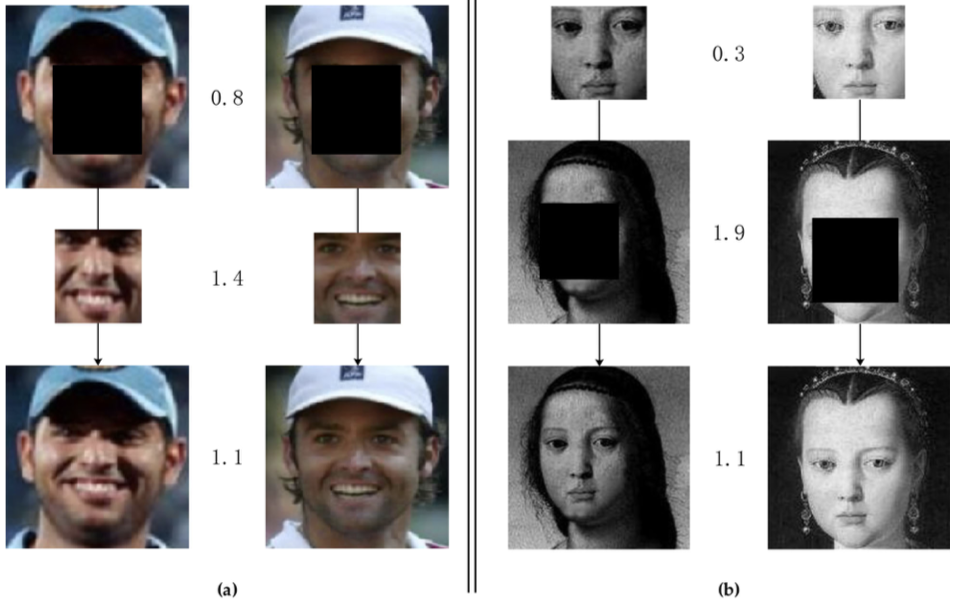
\includegraphics[width = 0.6\linewidth]{images/paper9/importance.png}
        \centering
        \caption{(a) Shows the importance of internal features and (b) shows the importance of external features. The values are the cosine distances.}
        \label{fig:features}
    \end{figure} 
\end{frame}

\begin{frame}{DATASET COLLECTION}
    One of the purposes of this paper is to create a dataset containing similar 
    faces called similar-face-dataset (SFD), in order to test the proposed 
    IE-CNN recognition model with other models. To create the dataset, the 
    following steps were performed:
    \begin{enumerate}
        \item \emph{Collecting The Suitable Data Source}: from LFW and CASIA-WebFace datasets.
        \item \emph{Determining the Similarity Between Two Faces Images}: with distance $L2$ on image vectors.
        \item \emph{Generating the Similar FaceDataset (SFD)}: with images classified in different Grades.
    \end{enumerate}
\end{frame}

\begin{frame}{IE-CNN NETWORK - ARCHITECTURE}
    This paper proposes IE-CNN model which contains two modules to 
    extract internal (local pathway) and external (global pathway) features. 
    The outputs, generated by both pathways, will be merged with a 
    concatenation operation to create a single feature map.
    \begin{figure}[h!]
        \centering
        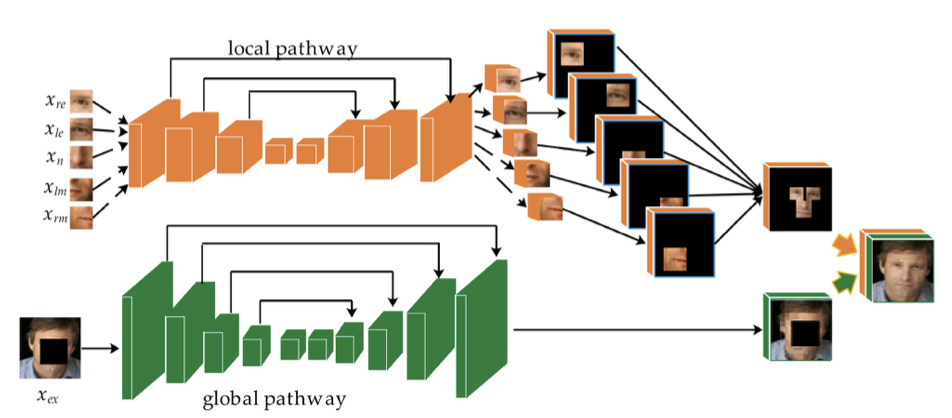
\includegraphics[width = 0.8\linewidth]{images/paper9/IE-CNN.png}
        \centering
        \caption{IE-CNN Architecture.}
        \label{fig:IE-CNN ARCHITECTURE}
    \end{figure}
\end{frame}

\begin{frame}{IE-CNN NETWORK - TRAINING}
    Triplets are used to train the network, each consisting of:
    \begin{enumerate}
        \item $x^o$ (\emph{original}): represents the image of the face of a single individual;
        \item $x^p$ (\emph{positive}): represents the remaining images of the same individual;
        \item $x^n$ (\emph{positive}): represent the images of the faces of the other different 
        individuals.
    \end{enumerate}
    The aim is to have smaller Euclidean distances between $x^o$ and $x^p$. The 
    search for these triplets can be traced back to an optimization problem.
    \begin{figure}[h!]
        \centering
        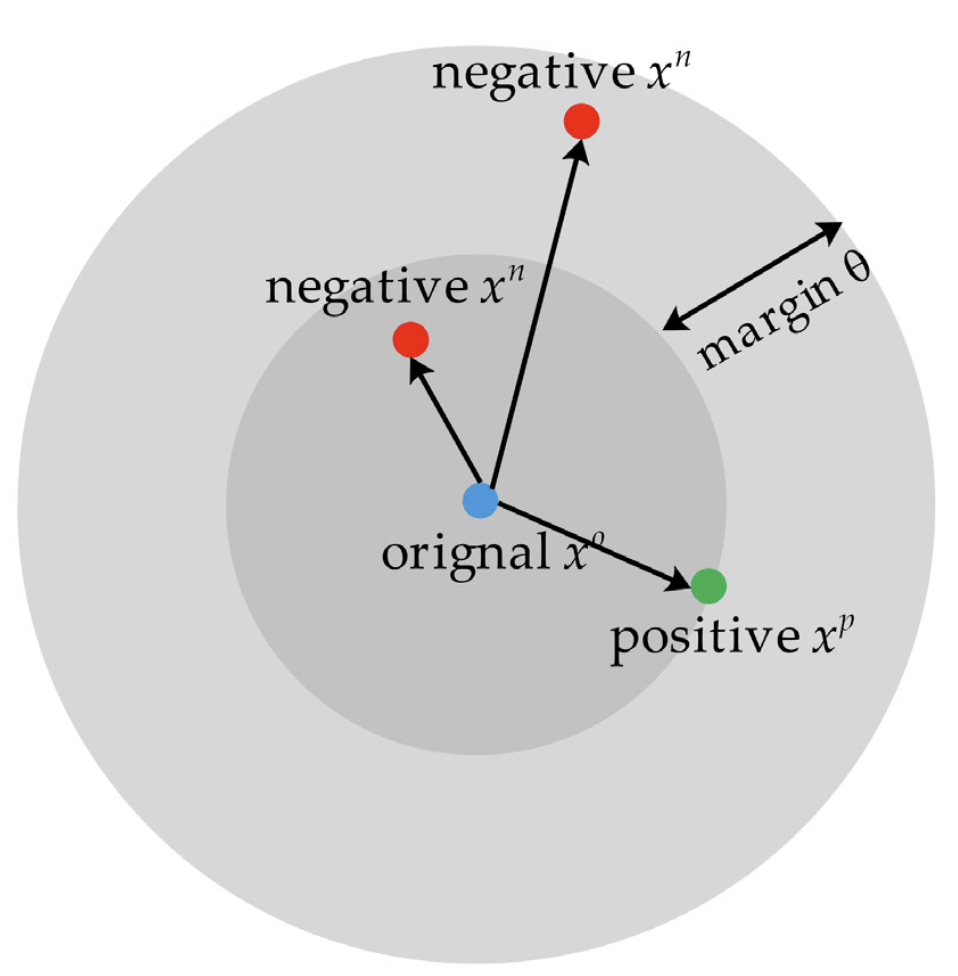
\includegraphics[width = 0.3\linewidth]{images/paper9/SET.png}
        \centering
        \caption{High-dimensional space.}
        \label{fig:HDS}
    \end{figure}
\end{frame}

\begin{frame}{EXPERIMENTAL - LFW and CASIA-WebFace datasets}
    \begin{minipage}{\linewidth}
        \centering
        \begin{minipage}{0.45\linewidth}
            \begin{figure}[h!]
                \centering
                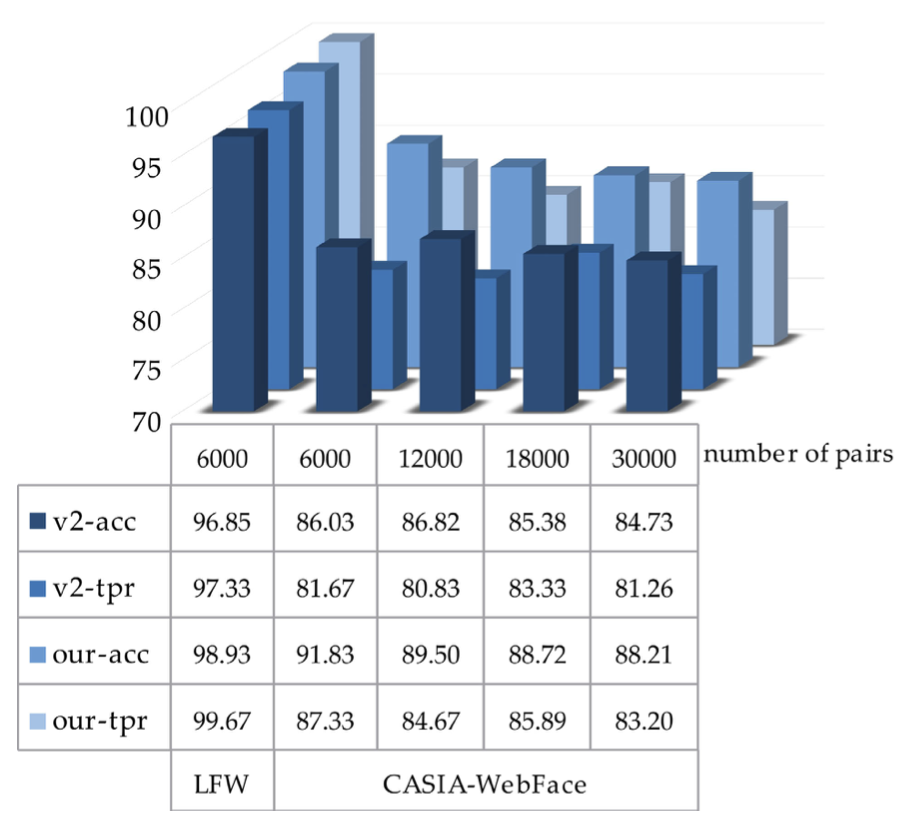
\includegraphics[width = \linewidth]{images/paper9/comparisonV2.png}
                \centering
                \caption{Comparison between v2 and the proposed methods on LFW and CASIA-WebFace datasets.}
                \label{fig:compareV2}
            \end{figure}
            \begin{table}[h!]
                \centering
                \begin{adjustbox}{max width=\textwidth}
                \begin{tabular}{|c|cc|cc|}
                    \hline
                    \multirow{2}{*}{Method} & \multicolumn{2}{c|}{LFW} & \multicolumn{2}{c|}{CASIA-WebFace}\\
                    & Top5-acc & Top1-acc & Top5-acc & Top1-acc\\
                    \hline
                    v2 & 96.96 & 93.63 & 85.97 & 78.24\\
                    \hline
                    proposed & \bfseries{99.20} & \bfseries{98.86} & \bfseries{93.31} & \bfseries{84.92}\\
                    \hline    
                \end{tabular}
                \end{adjustbox}
                \label{T12}
            \end{table}
        \end{minipage}
        \hspace{0.05\linewidth}
        \begin{minipage}{0.45\linewidth}
            In order to evaluate the proposed method, two metrics are used: sensitivity 
            (true positive rate) and accuracy. Another custom evaluation method used 
            is that of \emph{Top1 \& Top5 precision} (\%) (high is better). The 
            comparison is made with the Inception-Resnet-v2 model on the LFW and 
            CASIA-WebFace datasets.
        \end{minipage}
    \end{minipage}
    
\end{frame}

\begin{frame}{EXPERIMENTAL - Similar Face Dataset (SFD)}
    In this experiment, the performance of another method called DeepID2+ 
    was also verified. The reference dataset in this case is just SFD. The experiment 
    is conducted with images in which there are similar faces, divided by 
    degrees. Also in this case accuracy and sensitivity are the metrics considered.
    \begin{table}[h!]
        \centering
        \begin{adjustbox}{max width=\textwidth}
        \begin{tabular}{|c|ccccc|}
            \hline
            \multirow{2}{*}{Method} & \multicolumn{5}{c|}{Similar Face Dataset (SFD)}\\
            & \RN{1} & \RN{2} & \RN{3} & \RN{4} & \RN{5}\\
            \hline
            DeepID2+ acc. & 49.73 & 59.75 & 58.64 & 64.37 & 66.33\\
            DeepID2+ tpr. & 71.77 & 78.08 & 76.28 & 81.77 & 83.17\\
            \hline
            v2 acc. & 42.81 & 54.75 & 55.64 & 66.97 & 68.22\\
            v2 tpr. & 63.33 & 70.00 & 65.33 & 71.67 & 68.08\\
            \hline
            proposed acc. & \bfseries{78.29} & \bfseries{83.19} & \bfseries{82.19} & \bfseries{86.11} & \bfseries{86.40}\\
            proposed tpr. & \bfseries{79.17} & \bfseries{83.33} & \bfseries{79.67} & \bfseries{85.67} & \bfseries{84.67}\\
            \hline
        \end{tabular}
        \end{adjustbox}
        \caption{Comparison abount v2, DeepID+ and proposd methods on SFD dataset}
        \label{SFDCompMeth}
    \end{table}
\end{frame}

\begin{frame}{CONCLUSION}
    What appears strange is that the greater the similarity between two faces, 
    the lower the recognition accuracy achieved by all the models. Even if the 
    addition of external and internal features represent a benefit for the purpose 
    of recognition, at the computation level this operation turns out to be expensive 
    in the training phase even if it is lightened by the use of mini-batches 
    (triplet) and the various optimizations of the network.
\end{frame}